\chapter{Comparative Study}
\label{chap:comparative_study}

The version 1.2 of the \gls{tls} protocol was defined in \gls{rfc}5246 in August 2008 und has been in use many years. With the release of \gls{tls} 1.3 in August 2018 some security and speed improvements of the protocol have been implemented. The \gls{tls} 1.3 is defined in \gls{rfc}8446. In the following chapters the changes and differences of both \gls{tls} releases are examined and discussed.

\section{Handshake}
\label{sec:comparison_handshake}

As described in the chapter \ref{sec:handshake_protocol} the Handshake begins after the establishment of the \gls{tcp} connection between client and server. The goals of the handshake protocol are to authenticate the server and, optionally, the client; negotiate protocol version, cipher suites and extensions; derive authenticated encryption keys for the secure connection; ensure agreement on all negotiated parameters. \cite{Hassenstein}

\subsection{\gls{tls} 1.2 handshake}
\label{subsec:handshake1_2}

The figure \ref{fig:handshake1_2} shows the process of the full handshake in the \gls{tls} protocol 1.2 for simplicity only with authentication of the server. There will be more steps of the handshake in case of the mutual authentication when the client must be also authenticated by the server.

\begin{figure}[H]
	\centering
		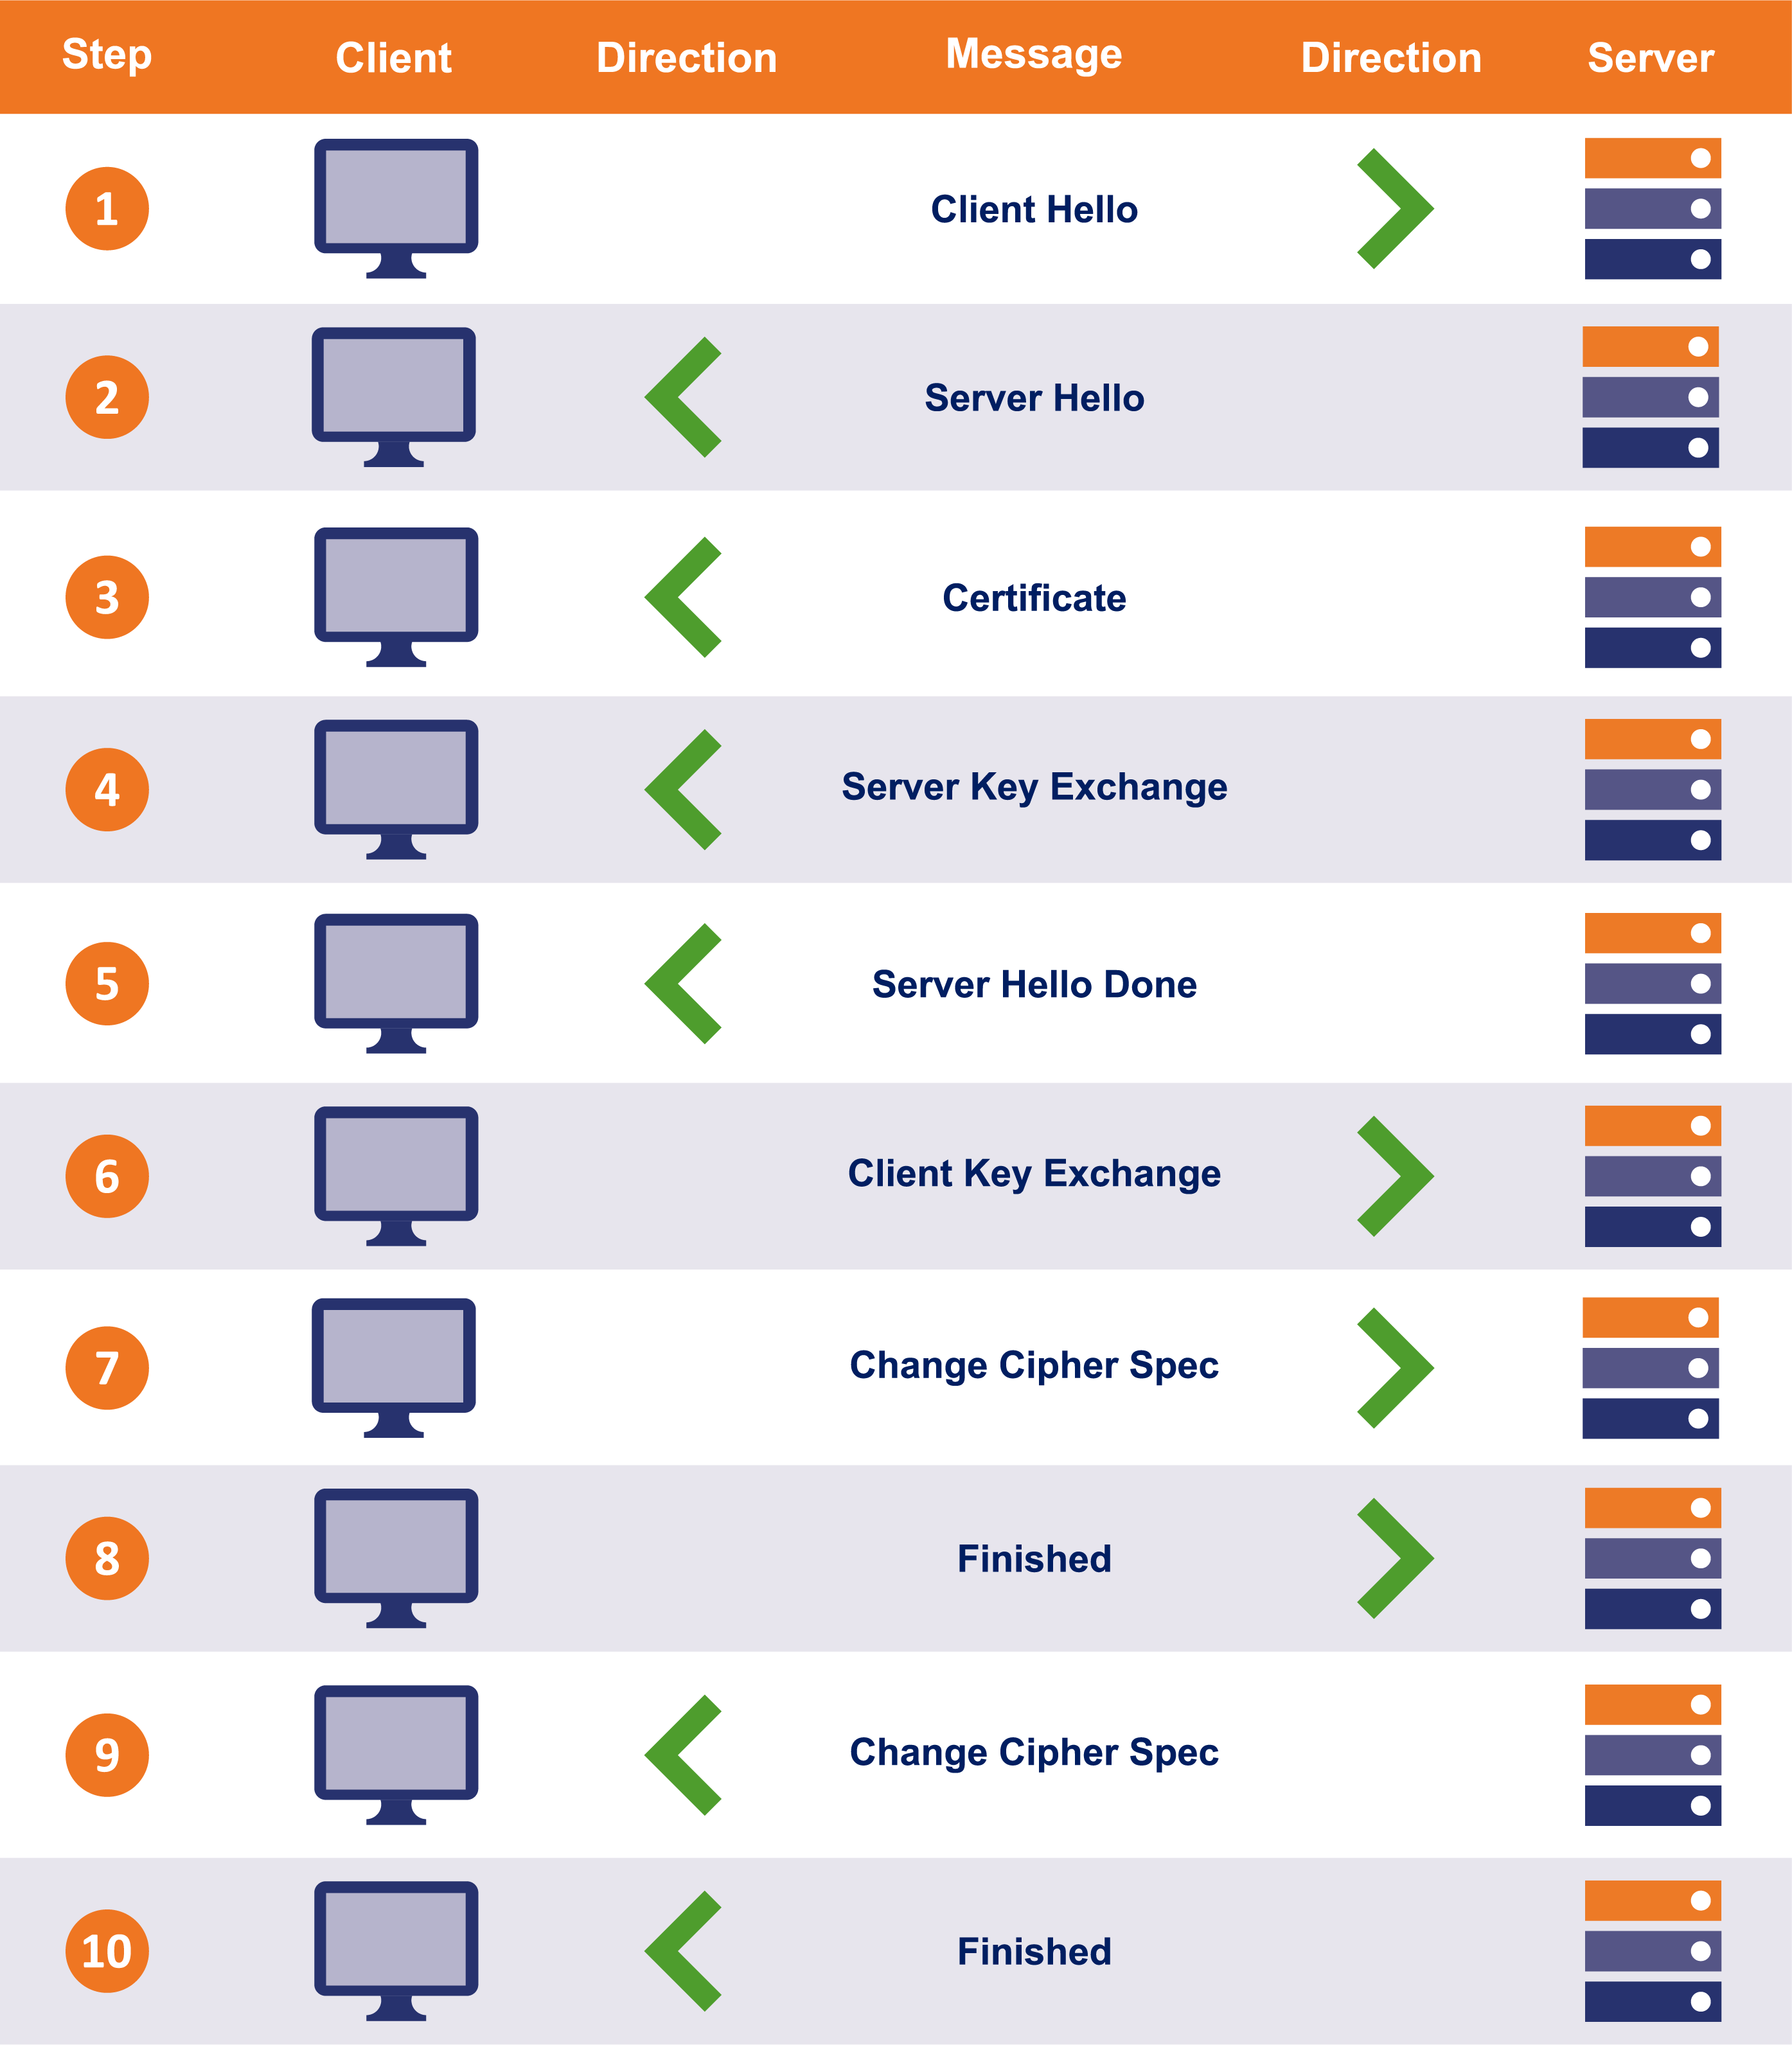
\includegraphics[scale=0.35]{images/handshake1_2.png}
	\caption{\gls{tls} 1.2 full handshake \cite{sslstore:handshake}}
	\label{fig:handshake1_2}
\end{figure}

\textbf{Step 1.} The 1th round of the handshake begins with the "client hello" message sent from the client to the server. This message includes the following cryptographic information:

\begin{itemize}
	\item CipherSuites - encryption algorithms supported by the client
	\item desired maximum of the protocol version
	\item random value generated on the client side
	\item session id
\end{itemize}

\textbf{Step 2.} Then the server responds with "server hello" message. The message consists of the following information:

\begin{itemize}
	\item CipherSuites chosen by the server from the "client hello" message
	\item protocol version supported by the server
	\item random value generated on the server side
	\item session id
\end{itemize}

\textbf{Step 3.} The server sends its X.509 certificate and its public key.

\textbf{Step 4.} This step is needed if the Diffie-Hellmann key exchange algorithm was negotiated between the client and the server at the steps 1 and 2. In this case the server transmits additional key materials in the "server key exchange" message.

\textbf{Step 5.} With the "server hello done" message the server notifies the client that it finished his steps and waits on the answer of the client.

\textbf{Step 6.} The client verifies the certificate sent by the server. Then it transmits to the server its key material in the key exchange message. 
At this point the client and the server can compute pre-master secret from key exchange messages. Using the pre-master secret with the nonces sent in the steps 1 and 2 they can generate the master key. Afterwards the client and the server derive a set of session keys from the master key that will be used to symmetrically encrypt the data.

\textbf{Step 7.} When the client derived the session key, it notifies the server about the change of the keys for the secure communication.

\textbf{Step 8.} With the message "Finished" the client signals to the server that it completed its tasks and is ready for the communication. This message includes \gls{mac} of the messages from the previous steps using the calculated master key, so that the server can verify the integrity of the handshake's messages.

\textbf{Step 9-10.} The server makes the same steps as the client in the steps 7-8 to switch the keys for the symmetric encryption and notifies the client with the message "finished". This message includes the \gls{mac} of the whole handshake log except "change cipher spec" messages from the steps 7 and 9. \cite{sslstore:handshake}\cite{Hassenstein}

Almost the whole communication in the handshake protocol flows in the clear text. Only beginning from the step 8, when the client finished his preparation for the secure communication, the next messages of the handshake will be encrypted.

\subsection{\gls{tls} 1.3 handshake}
\label{subsec:handshake1_3}

\begin{figure}[H]
	\centering
		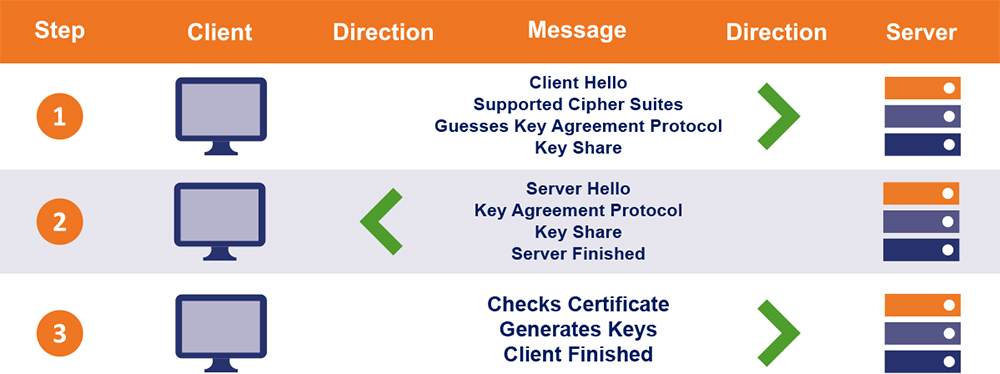
\includegraphics[scale=0.35]{images/handshake1_3.jpg}
	\caption{\gls{tls} 1.3 full handshake \cite{sslstore:handshake}}
	\label{fig:handshake1_3}
\end{figure}

\textbf{Step 1.} The \gls{tls} 1.3 handshake begins with the "client hello" message as in the \gls{tls} 1.2 handshake. In addition, the client sends also the following information with the message:

\begin{itemize}
	\item the list of the supported CypherSuites
	\item key share entries consisting of a named \gls{ecdh} group and an ephemeral public key
\end{itemize}

\textbf{Step 2.} The server respondes with the "server hello" message. In addition, it sends the following information:

\begin{itemize}
	\item chosen CypherSuite
	\item key share entries consisting of the chosen \gls{ecdh} group and its public key
	\item the certificate of the server
	\item "certificate verify" message containing a hash of all previous handshake messages signed with the private key of the server (the client afterwards verifies the signature with the public key from the server's certificate)
	\item "server finished" message
\end{itemize}

In case if the server does not support any of the proposed groups the server will request to retrying the handshake or will abort the connection with a fatal handshake\_failure alert.

\textbf{Step 3.} The client checks the certificate of the server. It generates keys from the key share of the server from the previous step. Afterwards the client sends the "client finished" message. \cite{Hassenstein}\cite{sslstore:handshake}

After the "server hello" message all handshake messages will be encrypted.
\cite{recorla}
\subsection{Discussion of \gls{tls} 1.2 and 1.3 full handshakes}
\label{subsec:comparison_handshake}

The \gls{tls} 1.2 handshake takes two round trips between the client and the server to complete the handshake. On average, this process requires 0.25 to 0.5 seconds.

The "server key exchange" and "client key exchange" messages have been removed from the \gls{tls} 1.3 handshake. The key exchange parameters and public keys will be sent in the key share extensions, that are added to the "client hello" and "server hello" messages. This keeps the 1.3 release compatible with the 1.2 version due to the remaining sending-order of messages.

Furthermore, the ChangeCipherSpec protocol has been removed in the 1.3 version. 

As a consequence of this missing protocol, the \gls{tls} 1.3 handshake involves only one round trip. This change results in reduced latency almost in half. As mentioned in the blog of The SSL Store a delay of half a second results in 20\% traffic decline \cite{sslstore:handshake}. That is why the performance improvement of the \gls{tls} protocol is a crucial change in the protocol.

Moreover, the privacy of the handshake protocol has been improved. In the 1.2 release of the \gls{tls} protocol almost all handshake messages are sent in the clear text except the last steps after the client sends "finished" message. On the contrary in the 1.3 version all information will be encrypted as early as possible, namely after "server hello" message. 

\section{Session resumption}
\label{sec:comparison_resumption}

The full handshake costs time, increase server load and cause connection latency. For performance improvement the session resumption can be used. With the "client hello" and "server hello" messages the session id can be saved and used to resume the previously established \gls{tls} session. Under this session id the client and the server store the master key and other details of the connection. In the next session they can transmit the session id and thus reuse the connection parameters. The following session data can be cached:
\begin{itemize}
\item master secret
\item protocol version
\item cipher suits
\item compression method
\item certificate
\end{itemize}
Because the session resumption is efficient it is supported per default in all major web browsers and web servers. But if it is not correctly implemented that can lead to vulnerabilities.

\subsection{Session resumption in \gls{tls} 1.2}
\label{subsec:resumption1_2}

The client and the server can set up a new connection by reusing the master key from the recent session cached on both ends in the one round-trip handshake. This kind of handshake is called abbreviated \gls{tls} handshake. The figure \ref{fig:resumption1_2} illustrates the process of the abbreviated handshake for the session resumption in the \gls{tls} 1.2.

\begin{figure}[H]
	\centering
		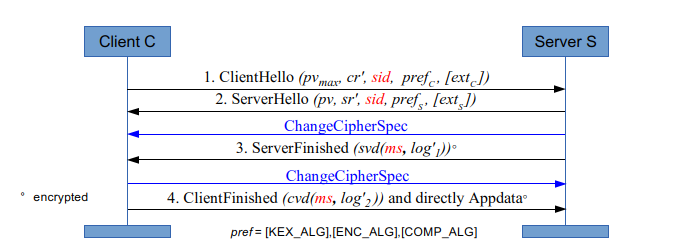
\includegraphics[scale=0.85]{images/resumption1_2.png}
	\caption{Abbreviated Handshake for Session Resumption in \gls{tls} 1.2 \cite{Hassenstein}}
	\label{fig:resumption1_2}
\end{figure}

In the "client hello" message the client sends to the server the session id from which the connection parameter can be used. As well a new random value (nonce) should be transmitted by the client. If the session has been cached the server responds in the "server hello" message with a new nonce and the same CipherSuites as in the previous handshake. Without waiting for the client's answer, the server immediately notifies the client about the changes of the key with the ChangeCipherSpec message and finishes its part of the handshake with \gls{mac} of the abbreviated handshake log in the encrypted "server finished" message. The client answers with its notification about the change of the key and completes the handshakes process with the "client finished" message containing a \gls{mac} of the whole abbreviated handshake log with the exception of ChangeCipherSpec messages. The both parties use the master key from the previous handshake and the new nonce to derive a set of session keys for the symmetric encryption of their communication.

The session resumption is also possible with the session ticket. In this case the client transmits the session ticket in the "client hello" message instead of the session id. The session ticket is a blob file created by the server and stored on the client side. This file contains all necessary detail of a connection and is encrypted with the key only known to the server. After the decryption of the ticket by the server the master key will be resumed for the derivation of session keys.

Figure \ref{fig:without-with-resume-1_2} demonstrates the efficiency of the session resumption. The abbreviated handshake is almost in half faster than the full handshake.

\begin{figure}[H]
	\centering
		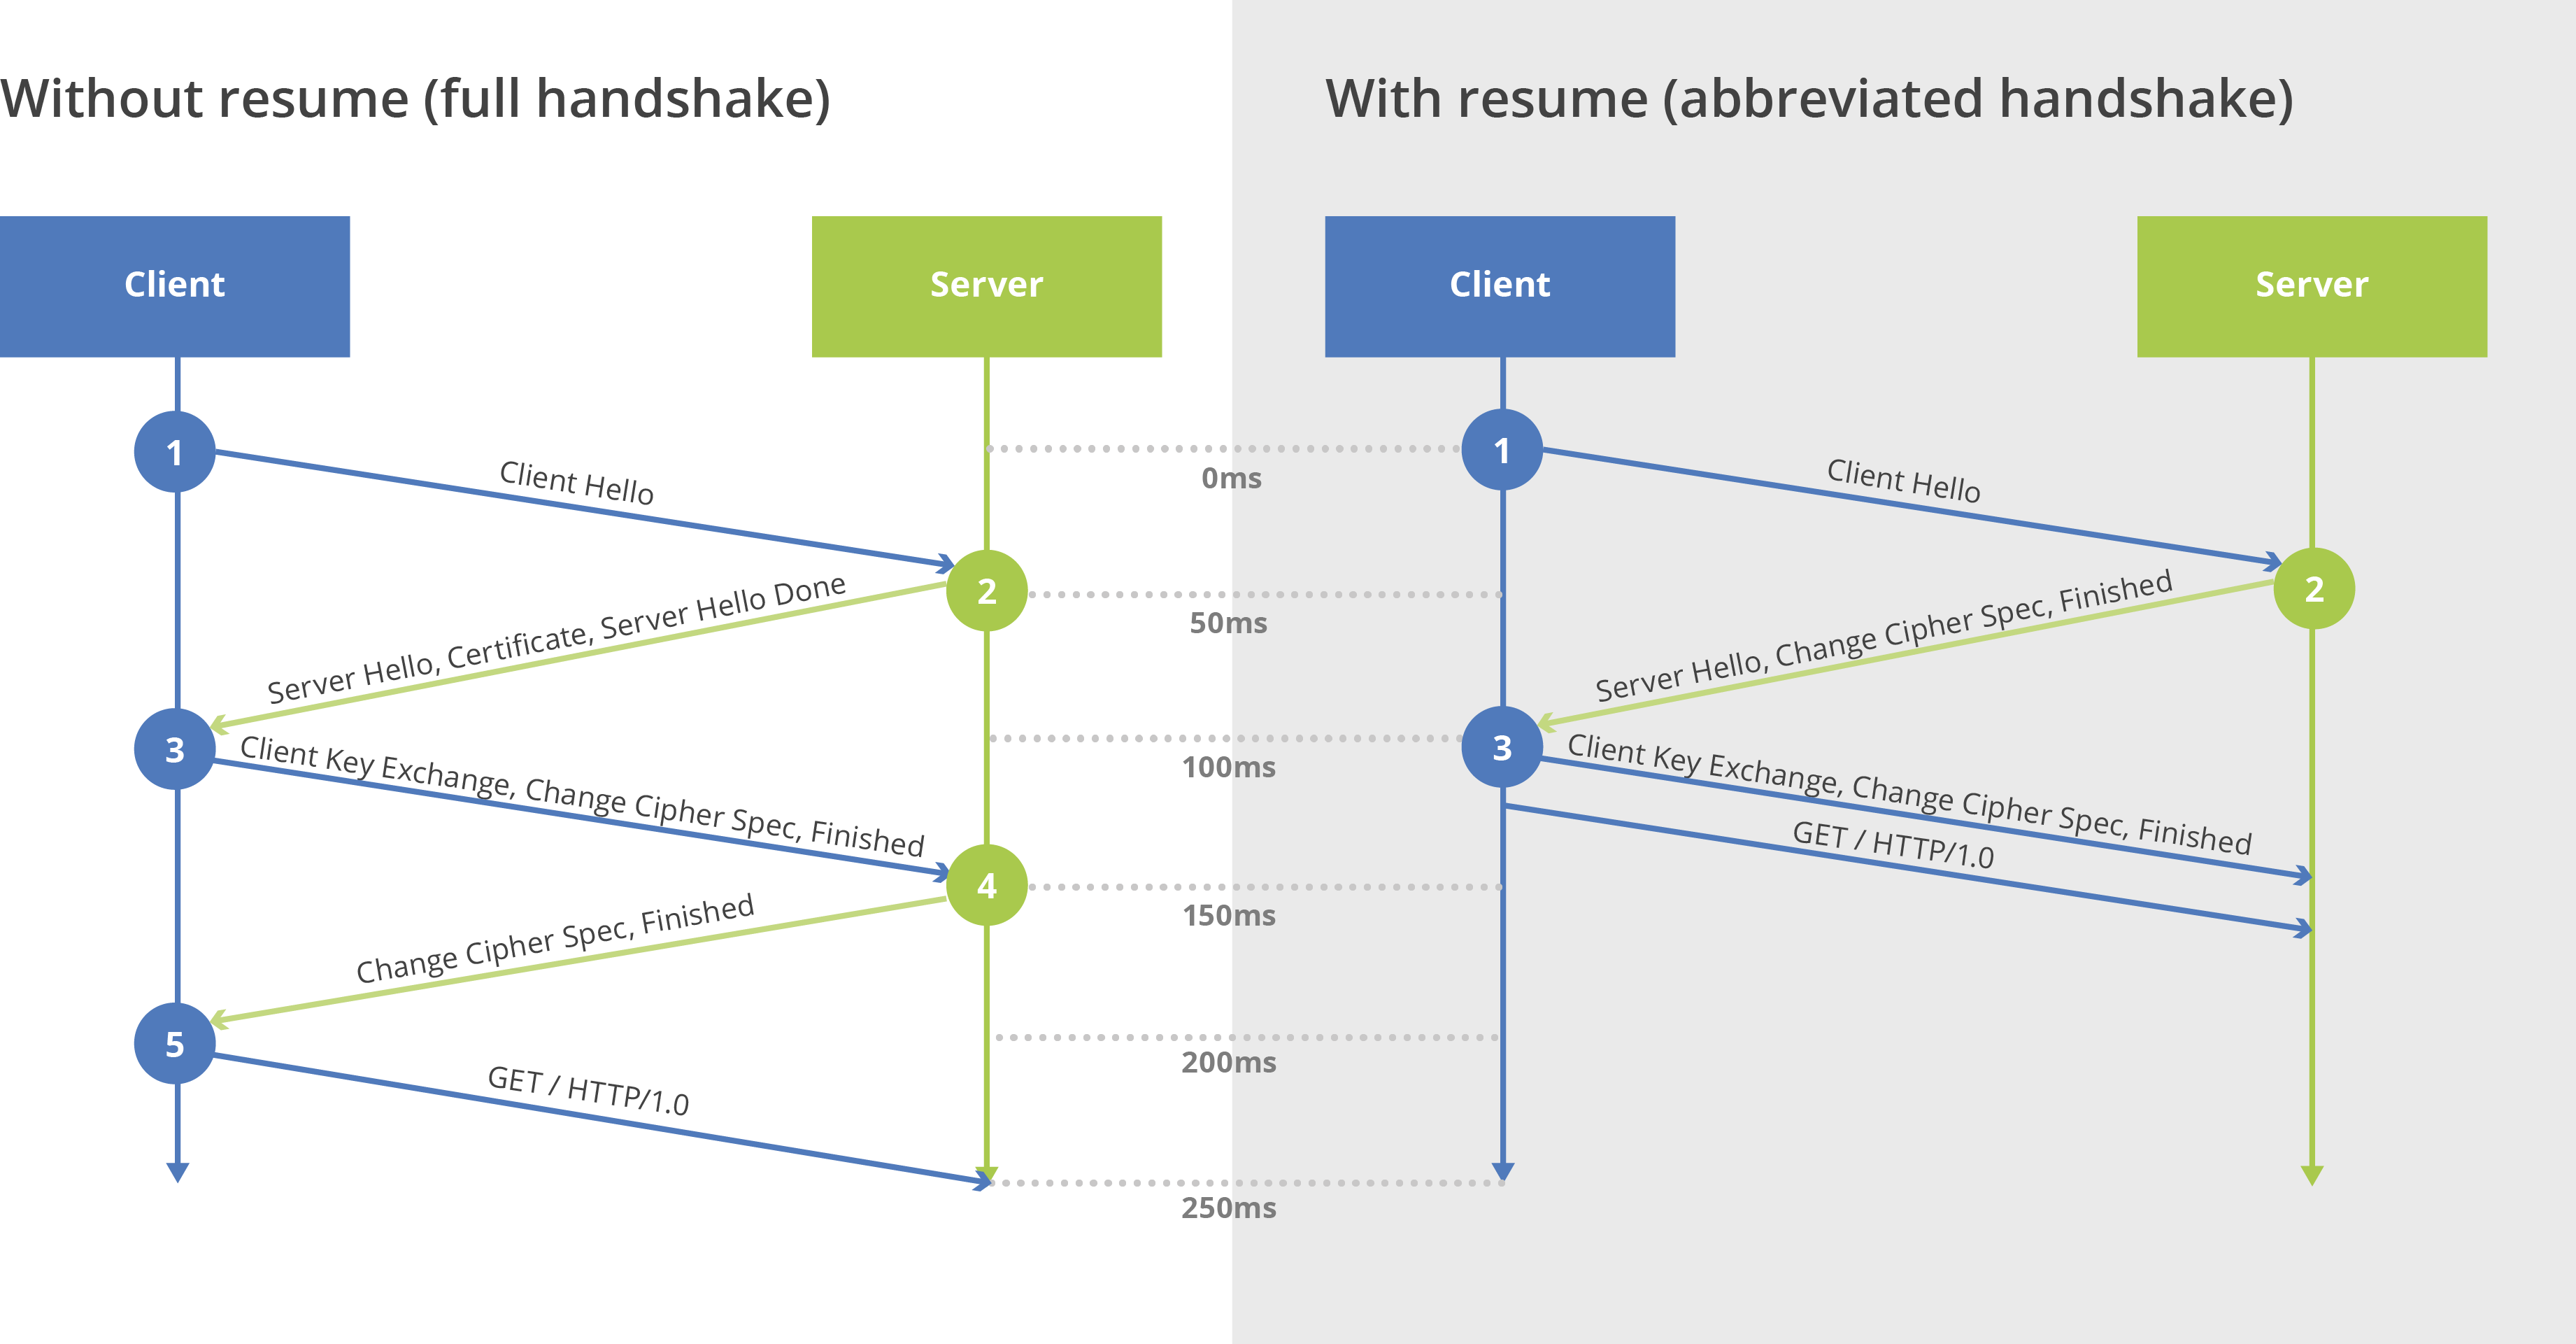
\includegraphics[scale=0.4]{images/without-with-resume-1_2.png}
	\caption{Full \gls{tls} handshake vs. abbreviated \gls{tls} handshake \cite{cloudflare:resume}}
	\label{fig:without-with-resume-1_2}
\end{figure}

\subsection{Session resumption in \gls{tls} 1.3}
\label{subsec:resumption1_3}

There are differences how the session resumption works in the release 1.3 of \gls{tls}. Figure \ref{fig:resumption1_3} illustrates the process of the handshake for the session resumption in \gls{tls} 1.3.

\begin{figure}[H]
	\centering
		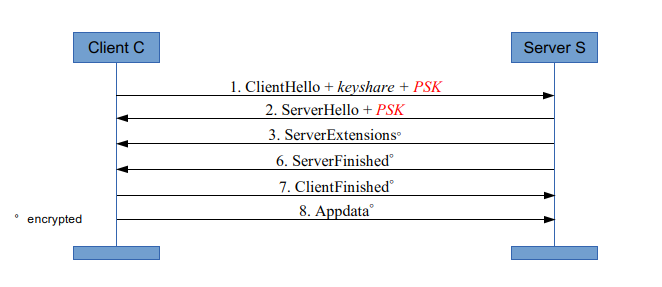
\includegraphics[scale=0.8]{images/resumption1_3.png}
	\caption{Handshake for Session Resumption in \gls{tls} 1.3 \cite{Hassenstein}}
	\label{fig:resumption1_3}
\end{figure}

A new method to resume the session is implemented in \gls{tls} 1.3. It is called pre-shared key (\gls{psk}) mode and replaces the usage of the session identifier or session ticket. An \gls{psk} identity is sent to the client by the server after the full handshake is completed. The \gls{psk} identity is a blob file containing database lookup keys or self-encrypted and self-authenticated values. It corresponds to a key derived from the handshake.

A \gls{psk}, that has been created during the handshake of the previous connection, can be presented by the client on the next visit. If it is needed to resume the session the client transmits \gls{psk} identities to the server. Then the server responds with the chosen \gls{psk} identity in the "server hello" message. The security context of this identity will be used in the new connection and the unique key derived from the previous connection can be used in the new one. 
The client can transmit the data to the server immediately in the first step together with the \gls{psk}. The data will be encrypted with the key derived from this \gls{psk}. \cite{ldapwiki:resumption}

\subsection{Discussion of the session resumption in \gls{tls} 1.2 and 1.3}
\label{subsec:discussion_resumption}
Though the performance of the session resumption in \gls{tls} 1.2 is very fast, it can lead to some security problems. Using the same session id during the resumption the same master secret is used. In case of compromised master key all resumed session will be revealed.

Using 0-\gls{rtt} handshake in \gls{tls} 1.3 does not provide perfect forward secrecy. It does also not protect against replay attack in the contrary to 1-\gls{rtt} where the server transmits a random value in each handshake.

Using 0-\gls{rtt} handshake in \gls{tls} 1.3 does not provide a perfect forward secrecy. It does also not protect against replay attack in the contrary to 1-\gls{rtt}, where the server transmits a random value in each handshake.
\cite{recorla}

\section{Cipher suites}
\label{sec:comparison_ciphersuits}

A cipher suite contains the key exchange and authentication algorithms for the handshake, the encryption and message authentication code (\gls{mac}) algorithm for the record protocol. The cipher suite contains different combinations of these algorithms.

\subsection{Cipher suites in \gls{tls} 1.2}
\label{subsec:ciphersuits1_2}

In the following the cipher suites for key exchange and the authentication in \gls{tls} 1.2 are described.

\subsubsection*{\gls{tls}\_\gls{rsa} (Static \gls{rsa})} 
The key exchange is based on the key transport with \gls{rsa} public-private keys.
If this cipher suite is used, the following computations and communications are made during the handshake:
\begin{itemize}
	\item for the pre-master secret, the protocol version is concatenated with the 46 bytes random value generated by the client
	\item the "server key exchange" message in step 4 of the full handshake is not used
	\item the client transmits in the "client key exchange" message in the step 6 the pre-master secret encrypted with the public key of the server taken from its certificate
	\item the server which decrypts the message, gets the pre-master secret 
	\item both parties derive the master secret from it and a set of session keys
\end{itemize}

The keyEncipherment option must be enabled in the key usage extension of the certificate of the server.
This cipher suite does not offer perfect forward secrecy. If an adversary gets the private key of the server, he can decrypt the pre-master secret from the client, compute all session keys and can then decrypt the whole communication with them.

\subsubsection*{\gls{dh}\_\gls{rsa}/\gls{dh}\_\gls{dss}}
The fixed Diffie-Hellman is used for the key exchange. The certificate of the server contains the \gls{dh} public key and is signed with \gls{rsa} or \gls{dss}.
The keyAgreement flag must be enabled in the key usage extension of the certificate.

The following computations are made during the handshake:
\begin{itemize}
	\item the "server key exchange" message in step 4 of the full handshake is not used
	\item the client transmits in the "client key exchange" message in step 6 - its value for \gls{dh} exchange is: \\ $\displaystyle kex_c = g^c \bmod p $ 
	\item the client and the server compute the pre-master secret as follows: $\displaystyle pms = g^{cs} \bmod p$
	\item both parties derive the master secret from the pre-master secret and a set of session keys
\end{itemize}

\subsubsection*{\gls{dhe}\_\gls{rsa}/DHE\_\gls{dss}}
The key exchange is based on the Ephemeral Diffie-Hellman, and the server authentication - on the \gls{rsa}/\gls{dss} signature.

The following computations are made during the handshake:
\begin{itemize}
	\item the "server key exchange" message is transmitted by the server in step 4
	\item the "server key exchange" message contains the parameters of a \gls{rsa} group and an ephemeral public key computed by the server
	\item the "server key exchange" message is signed with a private key of the server
	\item the client verifies the signature of the message with a public key from the certficate of the server
	\item the client transmits in the "client key exchange" message in step 6 its ephemeral public key, which is compatible with the parameters sent by the server
	\item the client and the server compute the pre-master secret
	\item both parties derive the master secret from the pre-master secret and a set of session keys
\end{itemize}

The digitalSignature flag must be enabled in the key usage extension defined in the certificate of the server.

\subsubsection*{EC\gls{dhe}\_\gls{rsa}}
The key exchange is based on the Ephemeral Diffie-Hellman using elliptic curves and the server authentication - on the \gls{rsa}/\gls{dss} signature.

The following computations are made during the handshake:
\begin{itemize}
	\item the "server key exchange" message is transmitted by the server in step 4 
	\item the "server key exchange" message contains the parameters of an elliptic curve and an ephemeral public key computed by the server
	\item the "server key exchange" message is signed with the private key of the server
	\item the client verifies the signature of the message with the public key from the certficate of the server
	\item the client transmits in the "client key exchange" message in step 6 its ephemeral public key, which is compatible with the parameters sent by the server
	\item the client and the server compute the pre-master secret
	\item both parties derive the master secret from the pre-master secret and a set of session keys
\end{itemize}

The digitalSignature flag must be enabled in the key usage extension of the server's certificate.

\subsubsection*{\gls{rsa}\_anon}
The key exchange is based on the Anonymous Diffie-Hellman. In this case neither the server nor the client is authenticated, both parties remain anonymous. But the communication with this cipher suite is vulnerable to the man-in-the-middle attacks.

The following computations are made during the handshake:
\begin{itemize}
	\item the server sends the "server key exchange" message in step 4 with the following value: $\displaystyle kex_s = g^s \bmod p $ 
	\item the client transmits in the "client key exchange" message in step 6 its value for DH exchange: \\ $\displaystyle kex_c = g^c \bmod p $ 
	\item the client and the server compute the pre-master secret as follows: $\displaystyle pms = g^{cs} \bmod p$
	\item both parties derive the master secret from the pre-master secret and a set of session keys
\end{itemize}

\subsubsection*{Cipher suites for encryption}

In the last years many attacks have been performed against commonly used cipher suites and their modes of operation in TLS 1.2. For instance the stream cipher RC4 is used though its weaknesses have been proved and it has been recognized as insecure. There are some attacks against CBC mode of AES encryption if it is not correct implemented.
The list of stream and block encryption algorithms are presented in Table{tab:comparison}.


\subsection{Cipher suites in \gls{tls} 1.3}
\label{subsec:ciphersuits1_3}

The cipher suite concept has been changed to separate the authentication and key exchange mechanisms.
For the key exchange in \gls{tls} 1.3 only \gls{dhe} and \gls{ecdhe} are used providing the perfect forward secrecy. Five elliptic curve groups and five \gls{dhe} groups from Galois field are predefined, that eliminates the risk of the unsecure implementation of \gls{tls} by the administrators and developers.

The following signature algorithms remain: 
\begin{itemize}
	\item \gls{eddsa} (Edwards-curve Digital Signature Algorithm)
	\item \gls{ecdsa} (Elliptic Curve Digital Signature Algorithm) and \gls{rsa}
\end{itemize}

The list of supported symmetric algorithms has been reduced to Authenticated Encryption with Associated Data (\gls{aead}) algorithms.
The weak cryptographic algorithms have been deprecated, such that using static \gls{rsa} in the key exchange, \gls{rcv} stream cipher, MD5 and SHA-1 hash functions. The compression of the plaintext before the applying of \gls{mac} is removed.
The whole list of the algorithms used in the release 1.3 is shown in table \ref{tab:comparison}.
\cite{recorla}
\section{Key derivation}
\label{sec:comparison_kdf}

For the key derivation in TLS 1.2 HMAC with SHA256 as pseudo-random function (PRF) is used. The PRF takes the pre-master key as an input for the master key derivation. \\
The key derivation funcitons habe been re-desired in TLS 1.3. The HMAC-based Extract-and-Expand Key Derivation Function (HKDF) is used as an underlying primitive \cite{Hassenstein}. It replaces PRF based on HMAC.


\section{Comparison: \gls{tls} 1.2 vs 1.3}
\label{sec:comparison}

The Table \ref{tab:comparison} illustrates a brief summarized comparison of both versions of \gls{tls}.

\begin{table}[H]
	\centering
		\begin{tabular}{lll} \toprule
			\textbf{Characteristic} & \textbf{\gls{tls} 1.2} & \textbf{\gls{tls} 1.3} \\ \midrule
			Round trip time of the full handshake & 2-\gls{rtt} & 1-\gls{rtt} \\ \midrule
			Encryption of handshake messages & at the end, & at the beginning, \\ 
			& from "client finished" message & after "server hello" message \\ \midrule
			Performance of the full handshake & 0.25-0.5 s & 0.2-0.3 s\\ \midrule
			Round trip time of the handshake & 1-\gls{rtt} & 0-RTT \\ 
			for session resumption \\ \midrule
			Session resumption method & session id or session ticket & pre-shared key identity \\ \midrule
			Key exchange algorithms & \gls{rsa} & \gls{dhe}\\ 
			& \gls{rsa}/\gls{dhe} & \gls{ecdhe}\\
			& ECDH \\
			& Secure Remote Password \\
			& Pre-shared key \\ \midrule
			Signature algorithms & \gls{rsa} & \gls{rsa}\\
			& \gls{dss} & \gls{ecdsa}\\
			& \gls{ecdsa} & \gls{eddsa} \\ \midrule
			Symmetric encryption algorithms & AES GSM, CCM, CBC  & AES GCM\\
			& ChaCha20-Poly1305 & AES CCM \\
			& 3DES & ChaCha20-Poly1305 \\
			& RC4 \\
			& Camellia et al.\\ \midrule
			Hash algorithms & MD5 & SHA-256 \\
			& SHA-256 & SHA-384 \\
			& SHA-384 \\ \midrule
			Key derivation & PRF based on HMAC & HKDF-Extract and \\
			& & HKDF-Expand functions \\ \midrule
			Compression & Yes & No \\ \midrule
			Renegotiation & Yes & No \\ \midrule
			Known attacks &  BEAST \\ & CRIME \\ & TIME\\ & BREACH\\ & POODLE\\ & Lucky 13\\ & FREAK\\ & Logjam\\ & DROWN \\ \midrule
		
		\end{tabular}
	\caption{Comparison of \gls{tls} 1.2 and \gls{tls} 1.3}
	\label{tab:comparison}
\end{table}

